\documentclass[a4paper, 11pt]{article}
\usepackage{comment} % enables the use of multi-line comments (\ifx \fi) 
\usepackage{fullpage} % changes the margin
\usepackage{enumitem}
\usepackage[T1]{fontenc}
\usepackage[polish]{babel}
\usepackage[utf8]{inputenc}
\usepackage{ragged2e}
\usepackage{graphicx}
\usepackage{datatool}
\usepackage{rotating}
\usepackage{placeins}
\usepackage{pdflscape}
\usepackage{float}
\usepackage{pdfpages}
\usepackage{xcolor} % for setting colors
\usepackage{verbatim}
\usepackage{listings}
\usepackage{color}
\usepackage{tikz}

\usepackage{pythonhighlight}

\usepackage{geometry}
\geometry{
a4paper,
total={190mm,270mm},
left=10mm,
top=10mm,
}

\usepackage{hyperref}
\hypersetup{
colorlinks,
citecolor=black,
filecolor=black,
linkcolor=black,
urlcolor=black
}

\definecolor{codegreen}{rgb}{0,0.6,0}
\definecolor{codegray}{rgb}{0.5,0.5,0.5}
\definecolor{codepurple}{rgb}{0.58,0,0.82}
\definecolor{backcolour}{rgb}{1,1,1}

\lstdefinestyle{mystyle}{
backgroundcolor=\color{backcolour},
commentstyle=\color{codegreen},
keywordstyle=\color{magenta},
numberstyle=\tiny\color{codegray},
stringstyle=\color{codepurple},
basicstyle=\ttfamily\footnotesize,
breakatwhitespace=false,
breaklines=true,
captionpos=b,
keepspaces=true,
numbers=left,
numbersep=5pt,
showspaces=false,
showstringspaces=false,
showtabs=false,
tabsize=2
}

\lstset{style=mystyle}

\title{Raport z wykonania ćwiczenia Neo4j}
\author{Jakub Płotnikowski}
\date{Styczeń 2020r.}


\begin{document}

    \maketitle
    \tableofcontents

    \newpage

    \section{Zainstalować serwer neo4j lokalnie}

    Zainstalowałem Neo4j Desktop Community:
    \url{https://neo4j.com/download-center/#community}

    Uruchamianie serwera Neo4j:
    \lstinputlisting[language=Python]{source_code/start_command.py}

    Serwer dostępny był pod adresem: \url{http://localhost:7474/browser/}

    \newpage

    \section{Wgrać bazę}

    Zadanie wykonałem w Pythonie, do każdego zadania dołączony kod źródłowy oraz rezultat działania

    \lstinputlisting[language=Python]{source_code/imports.py}

    \begin{center}
        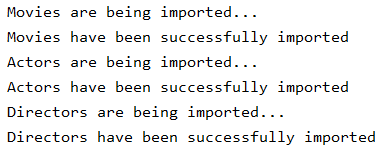
\includegraphics[scale=0.8]{images/imports.png}
    \end{center}

    \newpage

    \section{ Zaimplementować funkcję (wystarczy wykonać jedno zapytanie typu MATCH WHERE i wyświetlić wynik)}

    \lstinputlisting[language=Python]{source_code/task3.py}

    \begin{center}
        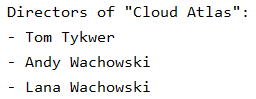
\includegraphics{images/task3.png}
    \end{center}

    \newpage

    \section{ Stworzyć kilka nowych węzły reprezentującychfilm oraz aktoróww nim występujących, następnie
    stworzyć relacje ich łączące (np. ACTED\_IN)}

    \lstinputlisting[language=Python]{source_code/task4.py}

    \begin{center}
        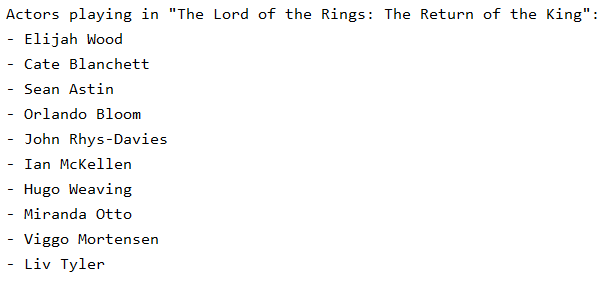
\includegraphics{images/task4.png}
    \end{center}

    \newpage

    \section{Dodać zapytaniem nowe właściwości nowo dodanych węzłów reprezentującychaktor (np. birthdate
    oraz birthplace).}

    \lstinputlisting[language=Python]{source_code/task5.py}

    \begin{center}
        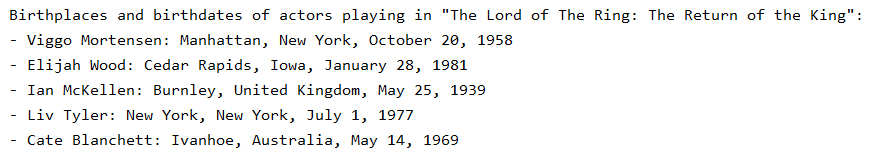
\includegraphics{images/task5.png}
    \end{center}

    \newpage

    \section{Ułożyć zapytanie, które zmieni wartość atrybutu węzłów danego typu, jeżeli innych atrybut węzła
    spełnia zadane kryterium}

    \lstinputlisting[language=Python]{source_code/task6.py}

    \begin{center}
        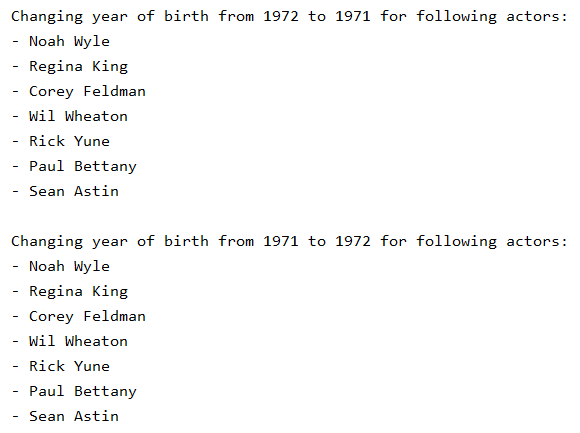
\includegraphics{images/task6.png}
    \end{center}

    \newpage

    \section{ Zapytanie o aktorów którzy grali w conajmniej 2 filmach (użyć collect i length) i policzyć średnią
    wystąpień w filmach dla grupy aktorów, którzy wystąpili w conajmniej 3 filmach.}

    \lstinputlisting[language=Python]{source_code/task7.py}

    \begin{center}
        
\includegraphics[scale=1.45]{images/task7.png}
    \end{center}

    \newpage

    \section{}

    \section{ Zmienić wartość wybranego atrybutu w węzłachna ścieżce pomiędzy dwoma podanymi węzłami}

    \lstinputlisting[language=Python]{source_code/task9.py}

    \begin{center}
        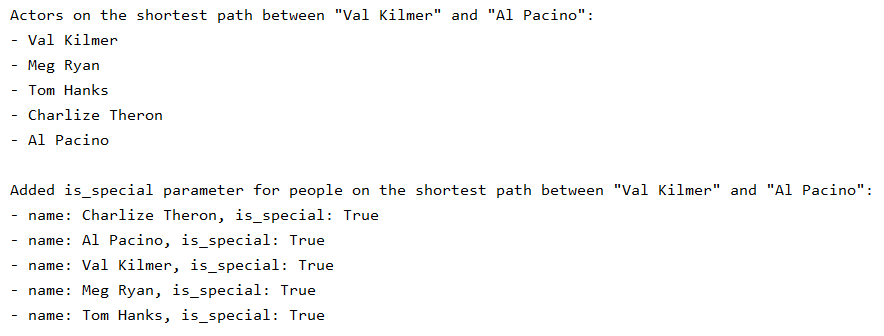
\includegraphics[scale=0.8]{images/task9.png}
    \end{center}

    \newpage

    \section{ Wyświetlić węzły, które znajdują się na 2 miejscu na ścieżkach o długości 4 pomiędzy dwoma
    wybranymi węzłami.}

    \lstinputlisting[language=Python]{source_code/task10.py}

    \begin{center}
        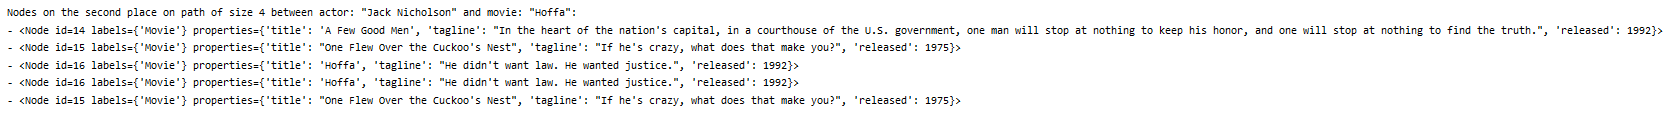
\includegraphics[scale=0.55]{images/task10.png}
    \end{center}

    \newpage

    \section{ Porównać czas wykonania zapytania o wybranego aktora bez oraz z indeksem w bazie nałożonym na
    atrybut name (DROP INDEX i CREATE INDEX oraz użyć komendy PROFILE/EXPLAIN).}

    Poniższe 2 screeny przedstawiają wykonanie zapytania EXPLAIN - o aktora Jacka Nicholsona.

    \subsection{Zapytanie bez indeksu}
    \begin{center}
        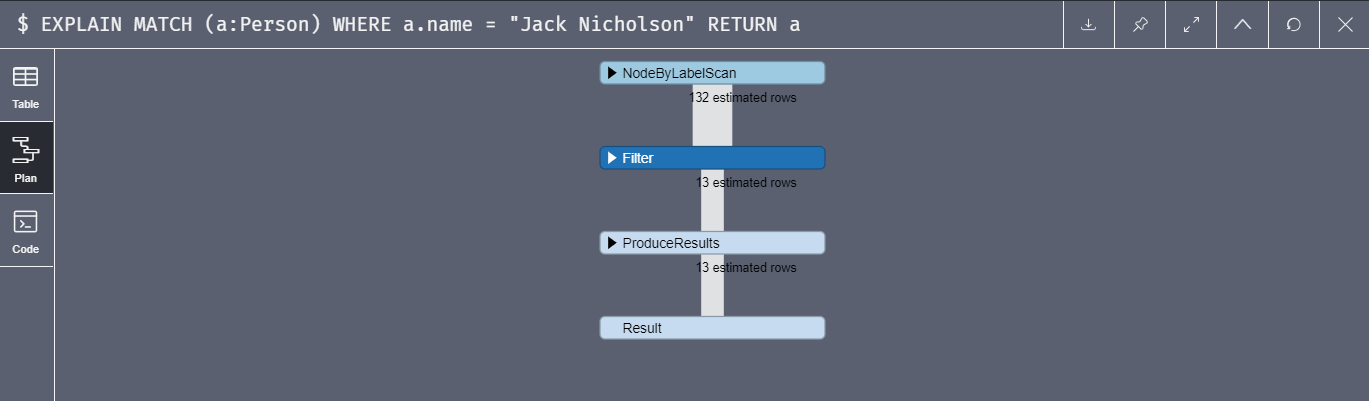
\includegraphics[scale=0.65]{images/explain_without_index.png}
    \end{center}

    Completed after 6 ms.

    \subsection{Zapytanie z indeksem}
    \begin{center}
        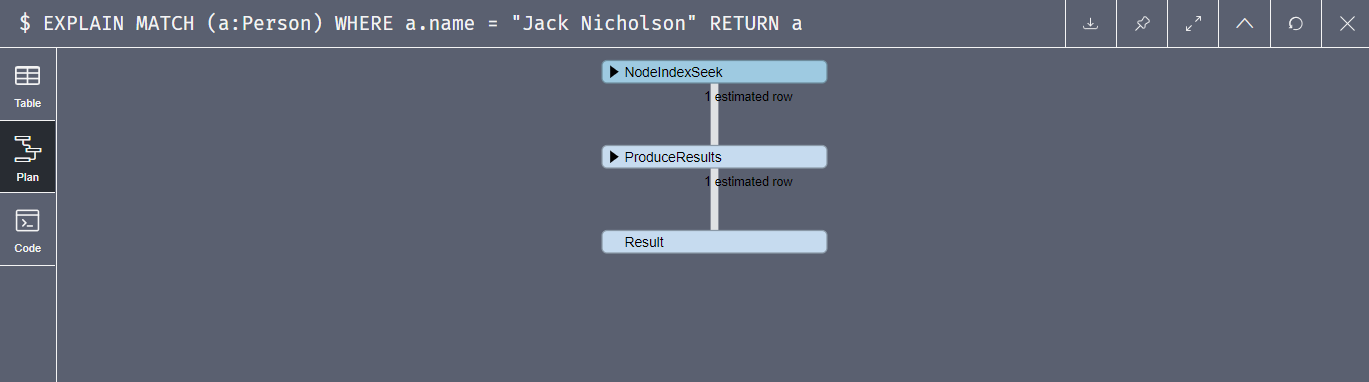
\includegraphics[scale=0.65]{images/explain_with_index.png}
    \end{center}

    Completed after 1 ms.

    \newpage

    \section{Spróbować dokonać optymalizacji wybranych dwóch zapytańz poprzednich zadań(załączyć
    przykłady w sprawozdaniu).}

    \lstinputlisting[language=Python]{source_code/task12.py}

    \newpage

    \section{Cały kod źródłowy programu}

    \lstinputlisting[language=Python]{source_code/neo4j.py}


\end{document}